\documentclass[]{article}
\usepackage[spanish.mexico]{babel}
\usepackage[T1]{fontenc}
\usepackage[utf8]{inputenc}
%\usepackageB.\\{lmodern}
\usepackage[a4paper]{geometry}

%\usepackage{natbib}
\usepackage{cite}


%Grafico de barras
\usepackage{pgfplots}

%Graficos e imagenes
\usepackage{graphicx}


\title{Formulario Máquinas Eléctricas}
\author{Pablo Vivar Colina}
%\date{Mayo 2018}

%EDADES, Para secundaria y prepa

\begin{document}
	
%	%\usepackage[top=2cm,bottom=2cm,left=1cm,right=1cm]{geometry}


\begin{titlepage}
     \begin{center}
	
\includegraphics[width=0.09\textwidth]{UNAM}\Large Universidad Nacional Autónoma de México
        	
\includegraphics[width=0.09\textwidth]{FI}\\[1cm]
        \Large Facultad de Ingeniería\\[1cm]
       % \Large División de Ciencias Básicas\\[1cm]
         \Large Laboratorio de Fundamentos de Control(6655)\\[1cm]
         %la clave antes era:4314
         \footnotesize Profesor: Salcedo Ubilla María Leonor Ing.\\[1cm]
        \footnotesize Semestre 2019-1\\[1cm]
        
       

        \Large Práctica No. 1\\[1cm]
        
           

\Large Introdcción MATLAB
        
         %Texto a la derecha
          \begin{flushright}
\footnotesize  Grupo 2\\[0.5cm]
\footnotesize Brigada: 4\\[0.5cm]
\footnotesize Rodrigo Adrián Martínez López\\[0.5cm]
\footnotesize Vivar Colina Pablo\\[0.5cm]
 \end{flushright}
    %Texto a la izquierda
          \begin{flushleft}
        \footnotesize Ciudad Universitaria Agosto de 2018.\\
          \end{flushleft}
         
          
        %\vfill
        %\today
   \end{center}
\end{titlepage}
 %agregar portada

\maketitle

%\tableofcontents  % Write out the Table of Contents

%\listoffigures  % Write out the List of Figures


\section{Entrehierro}

Sección del núcleo del transformador conformada por aire, es importante tenerla en cuenta ya que es un factor al momento de hacer cálculos correspondientes sobre los efectos magnéticos inducidos por las bobinas que conforman al transformador.\\

\section{Permanencia Entrehierro}

\begin{figure}[h!]
	\centering
	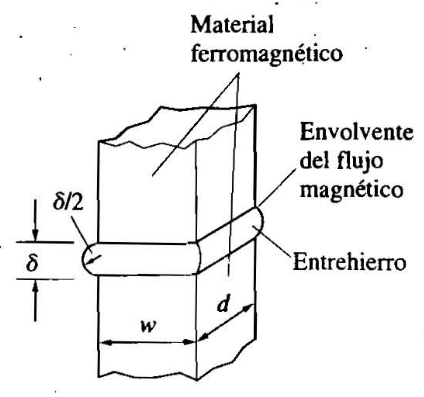
\includegraphics[width=0.3\textwidth]{EntreHierro}
	\caption{Diagrama de dimensiones entrehierro}
	\label{Entrehierro}
\end{figure}

\begin{figure}[h!]
	\centering
	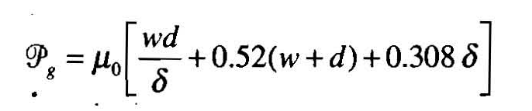
\includegraphics[width=0.3\textwidth]{PermanenciaEntrehierro}
    \caption{Permanencia entrehierro}
    \label{permEntrehierro}
\end{figure}

\section{Longitud media Núcleo de transformadores}

La longitud media de un núcleo del transformador es la sección lineal que se encuentra en el centro del laminado y tiene unidades de longitud, para contabilizarla se tiene que restar el entrehierro.\\


\section{Curvas de Magnetización}

\begin{figure}[h!]
	\centering
	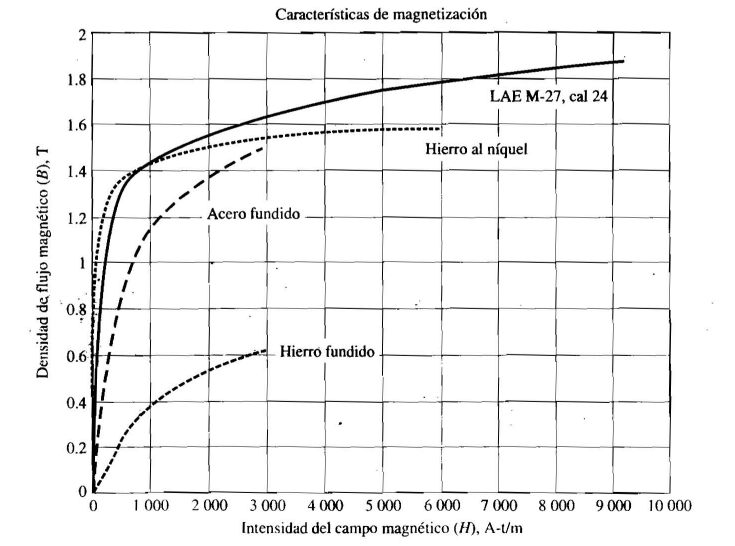
\includegraphics[width=1\textwidth]{curvasMagnetizacion}
	\caption{Curvas de Magentización para materiales ferromagnéticos típicos}
	\label{curvasMag}
\end{figure}




\section{Máquina de corriente directa}


\begin{figure}[h!]
	\centering
	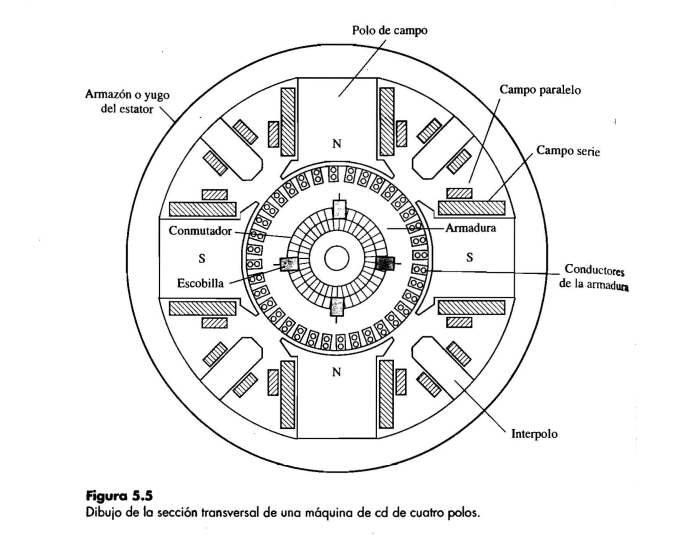
\includegraphics[width=1\textwidth]{maquina4polos}
	\caption{}
	\label{maq4polos}
\end{figure}

\begin{figure}[h!]
	\centering
	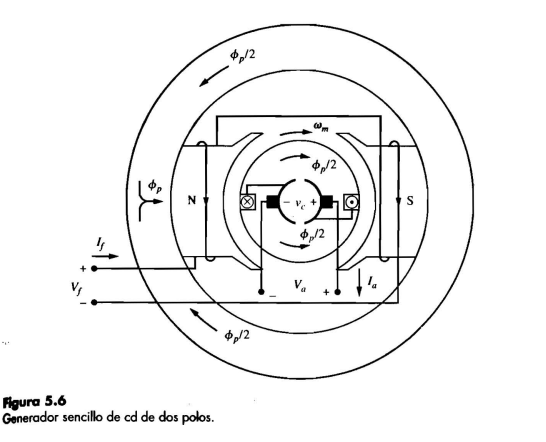
\includegraphics[width=1\textwidth]{maquinaCD2polos}
	\caption{}
	\label{maq2polos}
\end{figure}

\begin{figure}[h!]
	\centering
	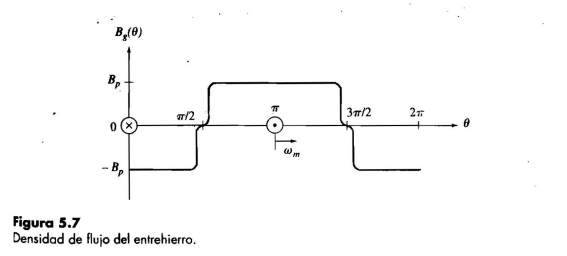
\includegraphics[width=1\textwidth]{densidadFlujoEntrehierro2polos}
	\caption{}
	\label{flujo2polos}
\end{figure}


\begin{figure}[h!]
	\centering
	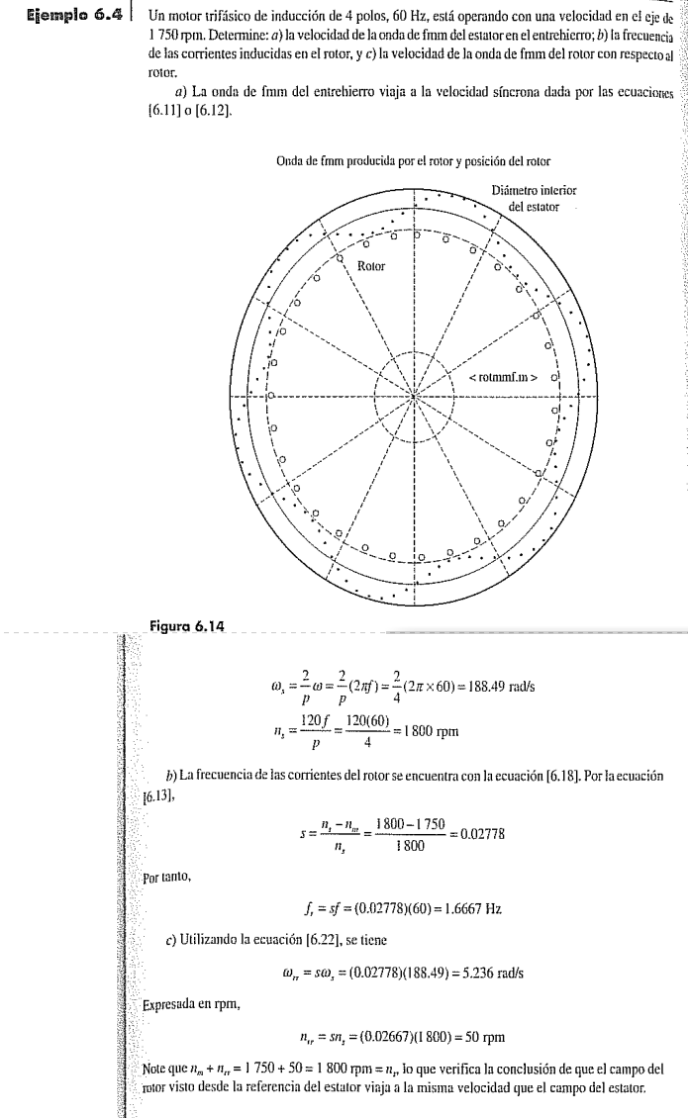
\includegraphics[width=1\textwidth]{maquinaInduccionEjemplo}
	\caption{Ejemplo maquina de inducción}
	\label{fig:maqInduccion}
\end{figure}





%\bibliographystyle{plain}
%\bibliography{Prac1}



\begin{thebibliography}{9}
	%\bibitem{latexcompanion} 
	%Michel Goossens, Frank Mittelbach, and Alexander Samarin. 
	%\textit{The \LaTeX\ Companion}. 
	%Addison-Wesley, Reading, Massachusetts, 1993.
	
	%\bibitem{einstein} 
	%Albert Einstein. 
	%\textit{Zur Elektrodynamik bewegter K{\"o}rper}. (German) 
	%[\textit{On the electrodynamics of moving bodies}]. 
	%Annalen der Physik, 322(10):891–921, 1905.
	
	
	%\bibitem{ebullicion} 
	 %Punto ebullición,
	%\\\texttt{http://www.cie.unam.mx/~ojs/pub/Liquid3/node8.html}
	
	
	%\bibitem{coccion} 
   %UnComo:Tiempo de cocción de los frijoles,
	%\\\texttt{https://comida.uncomo.com/articulo/tiempo-de-coccion-de-los-frijoles-34777.html}
\end{thebibliography}






\end{document}
